\section{Experimental Evaluation}\label{sec:eval}

\subsection{Methodology and What the Numbers Mean}\label{sec:metrics}
We report decision latency and throughput, on-chain gas, revocation exposure (requests accepted after the revocation instant), per-tier acceptance of legitimate and attacking requests, quorum behaviour, recall capacity and a degraded-mode scenario. Latencies are wall-clock times from a monotonic timer. Three limits apply throughout. (i) Testbed numbers are \emph{compute-bound}: they exclude network, block time and multi-node consensus. (ii) Sections~\ref{sec:scaling}--\ref{sec:outage_eval} use \emph{synthetic} devices, signals and attacks, so their detection-type results characterize policy mechanics under stated overlaps; Section~\ref{sec:real_eval} replaces the behavioural signal with detector scores computed on real TON\_IoT traffic, while posture and network context remain synthetic. (iii) One two-vCPU host was used.

\subsection{Testbed Performance and Repeated-Run Statistics}\label{sec:scaling}
Table~\ref{tab:results} gives one run per fleet size. Mean authorization latency is 0.120--0.197\,ms and registration 0.173--0.286\,ms; the two smallest fleets are slower (0.184 and 0.197\,ms against 0.120--0.127\,ms for $n\ge200$), probably from warm-up, which we did not isolate. Beyond $n=200$ latency is flat as the fleet grows eightfold, consistent with constant per-request cost dominated by one Ed25519 verification. Throughput is 3{,}700--6{,}200 decisions/s. Repeating $n=400$ thirty times gives a mean authorization latency of $0.133\pm0.013$\,ms (95\% CI 0.128--0.138) and registration $0.184\pm0.019$\,ms; over 20{,}000 sequential decisions the percentiles are p50 0.124, p95 0.188, p99 0.247 and p99.9 0.932\,ms, with a 4.3\,ms maximum attributable to scheduling or garbage collection. Intervals assume roughly normal run means and apply to this host.

\begin{table}[t]
\centering
\caption{Scaling results, one run per fleet size (latency in ms, throughput in ops/s)}
\label{tab:results}
\scriptsize
\begin{tabular}{@{}rrrrrr@{}}
\toprule
$n$ & Reg.\ lat. & AuthZ lat. & AuthZ p95 & Reg.\ tput & AuthZ tput \\
\midrule
50 & 0.286 & 0.184 & 0.216 & 3{,}477 & 3{,}812 \\
100 & 0.282 & 0.197 & 0.236 & 3{,}539 & 3{,}679 \\
200 & 0.256 & 0.125 & 0.148 & 3{,}906 & 5{,}909 \\
400 & 0.173 & 0.120 & 0.143 & 5{,}755 & 6{,}159 \\
800 & 0.177 & 0.127 & 0.162 & 5{,}645 & 5{,}804 \\
1{,}600 & 0.175 & 0.126 & 0.153 & 5{,}693 & 5{,}879 \\
\bottomrule
\end{tabular}
\end{table}

\subsection{On-Chain Cost: Measured EVM Gas}\label{sec:gas}
Table~\ref{tab:gas} lists gas measured over 50 devices on the Hardhat EVM; gas is deterministic given the state path (s.d.\ below 10). Registration costs about 215k gas and a full audited decision about 70k, of which one \texttt{ecrecover} and one new nonce slot are the main parts. Requests denied for replay (41.5k) or against a revoked device (39.3k) are cheaper because they exit early, while denials that occur after the oracle check cost as much as an allow. The industrial additions cost nothing visible: an ALLOW on a strict resource (70.4k), an anomaly-gate denial (70.2k), a strict-borderline denial (70.4k) and a below-threshold denial (70.2k) are all within 0.3\% of the base decision, since the extra checks are cheap comparisons. Anchoring a decision-log root costs 70.8k gas for the first anchor and 53.7k in steady state, which is 54 gas per decision at $B=1000$ decisions per root, about three orders of magnitude below the 70.4k of deciding each of them on-chain.

\begin{table}[t]
\centering
\caption{Measured gas per operation (Hardhat EVM, solc 0.8.24, 50 devices)}
\label{tab:gas}
\scriptsize
\begin{tabular}{@{}lrr@{}}
\toprule
\textbf{Operation} & \textbf{Mean gas} & \textbf{Std.} \\
\midrule
\texttt{registerDevice} & 214{,}950 & 8.9 \\
\texttt{suspendDevice} & 32{,}709 & 5.9 \\
\texttt{reinstateDevice} & 32{,}901 & 5.9 \\
\texttt{revokeDevice} & 58{,}824 & 5.9 \\
\texttt{evaluateAccess} (ALLOW) & 70{,}368 & 9.7 \\
\texttt{evaluateAccess} (STEP\_UP) & 70{,}413 & 8.0 \\
\texttt{evaluateAccess} (DENY, bad oracle sig.) & 70{,}143 & 8.3 \\
\texttt{evaluateAccess} (DENY, replay) & 41{,}526 & 9.7 \\
\texttt{evaluateAccess} (DENY, revoked) & 39{,}308 & 8.4 \\
\midrule
Deploy \texttt{IdentityRegistry} & 1{,}333{,}022 & -- \\
Deploy \texttt{ZeroTrustAccess} & 1{,}079{,}680 & -- \\
\texttt{definePolicy} (2 classes) & 97{,}805 & -- \\
\bottomrule
\end{tabular}
\end{table}

For capacity planning, a 30M-gas block (a typical default; PoA operators choose their own) holds at most $\lfloor 30\text{M}/70{,}369\rfloor=426$ audited decisions or 139 registrations. This is a gas-based upper bound, not a measured throughput (Section~\ref{sec:besu_eval} measures a much lower sustained rate on a real network), and it is the reason why only T2--T3 are decided on-chain. The in-process call latency including client-side signing was about 3\,ms per decision, an upper bound on pure EVM execution that says nothing about network or consensus delay.

\subsection{Hybrid Enforcement: Cost of the Fast Path}\label{sec:fast_eval}
We compare the contract model, which verifies one signature per decision (Track B), with the fast-path PEP, which verifies the device signature and the oracle attestation. Over 10 runs of 2{,}000 mixed T0/T2 requests, the contract model takes $0.134\pm0.020$\,ms (95\% CI 0.119--0.148) and the fast path $0.261\pm0.022$\,ms (CI 0.245--0.277). The fast path is therefore about twice as expensive \emph{in compute}, which is the expected cost of two verifications; it sustains roughly 3{,}800 decisions/s on one core. Its benefit is elsewhere: it needs no transaction, no gas and no block, and it keeps working when the ledger is slow. The compute comparison is thus a cost, not a gain, and the real advantage depends on the network and consensus latency that we did not measure.

\subsection{Tiered Policy: Legitimate Acceptance and Attack Acceptance}\label{sec:tiers_eval}
Table~\ref{tab:tiersres} runs 4{,}000 legitimate requests (5\% with a process upset) and 4{,}000 requests of each attack population through the four tiers, first with threshold alone and then with the full policy (gate and strict mode); eligibility is by device class, so the legitimate denominators shrink with the tier (4{,}000, 3{,}713, 1{,}145, 858). Fig.~\ref{fig:iiotres}(a) shows the same data graphically.

\begin{table}[t]
\centering
\caption{Per-tier results: legitimate requests allowed and attacker requests accepted (\%), threshold alone $\to$ full policy ($\theta$ min.\ trust, $g$ anomaly gate)}
\label{tab:tiersres}
\scriptsize
\setlength{\tabcolsep}{2.2pt}
\begin{tabular}{@{}lccrrr@{}}
\toprule
\textbf{Resource} & $\theta$ & $g$ & Legit. & Stealthy & Spoof \\
\midrule
telemetry.read (T0) & 0.50 & 1.00 & 100.0$\to$100.0 & 100.0$\to$100.0 & 100.0$\to$100.0 \\
historian.write (T1) & 0.55 & 0.60 & 100.0$\to$100.0 & 100.0$\to$100.0 & 100.0$\to$74.7 \\
plc.setpoint.write (T2) & 0.70 & 0.30 & 99.9$\to$97.8 & 98.5$\to$60.9 & 100.0$\to$0.0 \\
plc.firmware.update (T3) & 0.78 & 0.20 & 96.0$\to$94.8 & 52.2$\to$13.6 & 52.4$\to$0.0 \\
\bottomrule
\end{tabular}
\end{table}

Four observations follow. First, naive compromise is denied everywhere (0\% accepted at all tiers), so it does not test the design. Second, at T0 an attacker that spoofs signals is accepted 100\% of the time under any policy: this is by design, since T0 is read-only telemetry and we chose not to spend verification effort there, but it means T0 data can be read by a compromised device that keeps looking normal. Third, the gate and strict mode matter exactly where consequences are high: at T2 the full-spoof attacker falls from 100\% to 0\% accepted and the stealthy attacker from 98.5\% to 60.9\%; at T3 from 52.4\% to 0\% and from 52.2\% to 13.6\%. Fourth, this has a price. Legitimate allowance drops from 99.9\% to 97.8\% at T2 and from 96.0\% to 94.8\% at T3 (and 5.2\% of legitimate T3 requests are denied outright), because upset requests exceed the gate and strict mode refuses borderline scores. A plant would decide whether those denials are acceptable for setpoint and firmware writes, where a second confirmation is usually welcome, and the next experiment shows the trade-off.

A short ablation of the trust signals, run in the base design, adds that the full score separates partial and stealthy mimicry with AUC 0.993 and 0.895 whereas dropping the behavioural signal leaves both at AUC 0.499--0.500, so the behavioural signal is the only one that separates mimicry from legitimate traffic in this setup; posture and network are drawn from the same ranges for both populations in the synthetic fleet, so removing them \emph{raises} AUC, which argues for adaptive rather than fixed weighting and should not be read as evidence that real posture is uninformative.

\subsection{Sensitivity to the Anomaly Gate}\label{sec:gate_eval}
Fig.~\ref{fig:iiotres}(b) sweeps the gate level from 0.15 to 0.60 for legitimate upset rates of 5\% and 15\% (0\% gives no false denials by construction). Under a 5\% upset rate, a gate of 0.30 blocks 40.1\% of stealthy mimicry and 100\% of full spoofing while denying 2.3\% of legitimate requests. Tightening to 0.25 and 0.20 raises the stealthy block rate to 60.4\% and 80.4\% at 3.1\% and 3.8\% legitimate denials, and 0.15 blocks all of it at 4.6\%. Loosening to 0.40 blocks no stealthy attacker and lets 25\% of full spoofing through, rising to 74\% at 0.60. At a 15\% upset rate the same gates deny 7.4\% (0.30) and 12.2\% (0.20) of legitimate requests. The gate is thus a genuine trade-off whose operating point depends on how noisy legitimate behaviour is, and because the attack range $[0.15,0.40]$ is built to overlap legitimate upsets, no gate separates them completely; an attacker who keeps its anomaly below the gate is accepted, as Proposition~\ref{prop:bound}(d) predicts.

\subsection{Evaluation on Real Traffic: TON\_IoT}\label{sec:real_eval}
The synthetic study fixes the anomaly distributions by hand, so we repeat the central experiments with the anomaly signal $A$ produced by detectors on a public dataset. We use the TON\_IoT collection, which provides labelled IIoT telemetry \cite{alsaedi2020ton} and labelled network flows \cite{moustafa2021network}; the heterogeneity of its features and attack types is analysed in \cite{booij2022ton}. The dataset licence grants free use for academic research on condition that the dataset papers are cited. We used four telemetry files (Fridge, Modbus, Thermostat, Weather) and the network file (211{,}043 flows, of which 190{,}474 remain after removing 20{,}569 exact duplicates; nine attack types plus normal traffic).

\emph{Method.} Features exclude IP addresses and source ports, and for telemetry exclude dates and times, because normal and attack records were collected on different days. A gradient-boosted classifier (supervised) and an Isolation Forest trained on normal records only (unsupervised) are evaluated on a stratified 70/30 split repeated over five seeds. To approximate attacks unseen at training time, we also train the classifier with one attack type left out and score that type (seed 11). The classifier's attack probability is used as $A\in[0,1]$. Legitimate requests carry the score of a normal test flow, attackers carry the score of an attack flow and spoof posture and network context to 1 (the full-spoof attacker of Section~\ref{sec:devsim}); posture, network context and the reliability warm-up stay synthetic, and because the files share no device identifier, assigning a flow-derived score to a device is arbitrary. The four tiers of Table~\ref{tab:tiers} are used unchanged.

\emph{Telemetry alone is a weak signal.} Table~\ref{tab:telemetry} shows that only the Weather file separates attacks from normal records usefully (supervised AUC 0.972, Isolation Forest 0.819); Modbus gives 0.623 and 0.498, and Thermostat and Fridge are close to chance (0.513 and 0.531 supervised). The Fridge result requires a warning: before whitespace stripping, one column (\texttt{temp\_condition}) carries label-specific padding that gives a perfect AUC of 1.0, an encoding artefact that has nothing to do with device behaviour, so we strip all strings before training. We did not investigate why most telemetry is uninformative; one plausible reading is that the attacks target the services around a device rather than the physical readings it reports. The practical consequence is that a behavioural signal for a plant should come from traffic, not only from sensor values.

\begin{table}[t]
\centering
\caption{Detectability of attacks from TON\_IoT telemetry (five seeds, 70/30 split, after de-duplication)}
\label{tab:telemetry}
\scriptsize
\begin{tabular}{@{}lrrrr@{}}
\toprule
File & Rows & Att.\% & Sup. AUC & IF AUC \\
\midrule
Fridge & 37{,}110 & 67 & 0.531 & 0.484 \\
Modbus & 17{,}792 & 78 & 0.623 & 0.498 \\
Thermostat & 32{,}350 & 55 & 0.513 & 0.497 \\
Weather & 39{,}260 & 62 & 0.972 & 0.819 \\
\bottomrule
\end{tabular}
\end{table}

\emph{Network flows are a strong signal, with a caveat.} On flows the supervised classifier reaches AUC 0.9999 (s.d.\ below $10^{-4}$) and the Isolation Forest $0.916\pm0.004$, ranging from 0.813 (DDoS) to 0.956 (password attacks) by type. The near-perfect supervised value should be read as an upper bound: random splits of a benchmark whose attacks come from a few source hosts are optimistic, which is why we also test held-out types. With an attack type withheld, the AUC against normal traffic stays at 0.990--1.000, but the share of that type's flows scored above 0.5 falls to 65.4\% for ransomware and 73.7\% for man-in-the-middle, against 93--100\% for most others. Legitimate flows are overwhelmingly scored near zero (median 0.0003), but the tail is heavy: the 99th percentile is 0.27 and the 99.9th is 0.96, so any gate cuts into some legitimate traffic (see the gate sweep below).

\emph{Policy on real scores.} Table~\ref{tab:realpolicy} gives the percentage of attacker requests accepted, averaged over the nine attack types and, in the worst-case columns, for the single worst type, with threshold alone (Thr.) and with the full policy (gate and strict mode). Four findings follow. First, the full policy costs legitimate traffic little: allowance falls from 99.7, 99.5 and 99.0\% to 99.6, 98.8 and 98.4\% at T1, T2 and T3. Second, for attack types seen in training, the gate matters at T1 (mean acceptance 100\% $\to$ 0.7\%, worst 4.9\%, man-in-the-middle), whereas at T2 and T3 the high thresholds already reject nearly all such flows (1.1\% and 0.6\% with threshold alone), because a real detector scores them near 1 and Proposition~\ref{prop:bound}(d) then gives $T\approx0.7$ or below. This corrects the synthetic study, in which the stealthy population was built to sit at $A\le0.4$ and therefore overstated how often the threshold alone fails on seen attacks. Third, for held-out types, residual acceptance grows to 11.9\% (T1), 7.9\% (T2) and 6.6\% (T3) on average, and to 41.6\%, 33.9\% and 35.8\% for the worst type (ransomware), so a policy that depends on a detector inherits the detector's blind spots. Fourth, an adaptive attacker that can observe the detector and send only its best-scoring flows is much more dangerous: if it can send only the lowest-scoring 10\% of a held-out type's flows, mean acceptance at T1--T3 is 59.4, 37.9 and 29.0\%, and 76.5, 74.7 and 58.2\% for the best 1\%, with some types always accepted. We assume here that the attacker can query the detector and craft traffic with a chosen score, which is a strong capability, so these numbers describe a worst case rather than a typical one.

\begin{table}[t]
\centering
\caption{Attacker requests accepted (\%) with real TON\_IoT anomaly scores: mean over nine attack types and worst single type; threshold alone (Thr.) versus full policy}
\label{tab:realpolicy}
\scriptsize
\begin{tabular}{@{}llrrrr@{}}
\toprule
Scenario & Tier & Thr.\ mean & Full mean & Thr.\ worst & Full worst \\
\midrule
Seen types & T1 & 100.0 & 0.7 & 100.0 & 4.9 \\
 & T2 & 1.1 & 0.4 & 7.5 & 2.3 \\
 & T3 & 0.6 & 0.3 & 3.9 & 1.5 \\
\midrule
Held-out types & T1 & 100.0 & 11.9 & 100.0 & 41.6 \\
 & T2 & 15.9 & 7.9 & 51.5 & 33.9 \\
 & T3 & 9.3 & 6.6 & 36.7 & 35.8 \\
\midrule
Held-out, best 10\% & T1 & 100.0 & 59.4 & 100.0 & 100.0 \\
 & T2 & 64.1 & 37.9 & 100.0 & 100.0 \\
 & T3 & 49.3 & 29.0 & 100.0 & 100.0 \\
\midrule
Held-out, best 1\% & T1 & 100.0 & 76.5 & 100.0 & 100.0 \\
 & T2 & 87.4 & 74.7 & 100.0 & 100.0 \\
 & T3 & 76.0 & 58.2 & 100.0 & 100.0 \\
\bottomrule
\end{tabular}
\end{table}

Sweeping the gate on the real scores, a gate of 0.05 denies 3.6\% of legitimate flows and blocks 100\% of seen and 99.4\% of held-out attack flows; 0.30 denies 1.0\% and blocks 99.9\% and 94.6\%; 0.70 denies 0.3\% and blocks 99.7\% and 88.6\%; and 0.90 denies 0.2\% and blocks 99.5\% and 82.9\%. The real-score gate thus has a far better operating region than the synthetic one, because real attack scores are bimodal, but it degrades on unseen attack types. Detector hyper-parameters were left at library defaults, and the tier thresholds and gates are those fixed earlier for the synthetic study; none was tuned on these results.

\begin{figure*}[t]
\centering
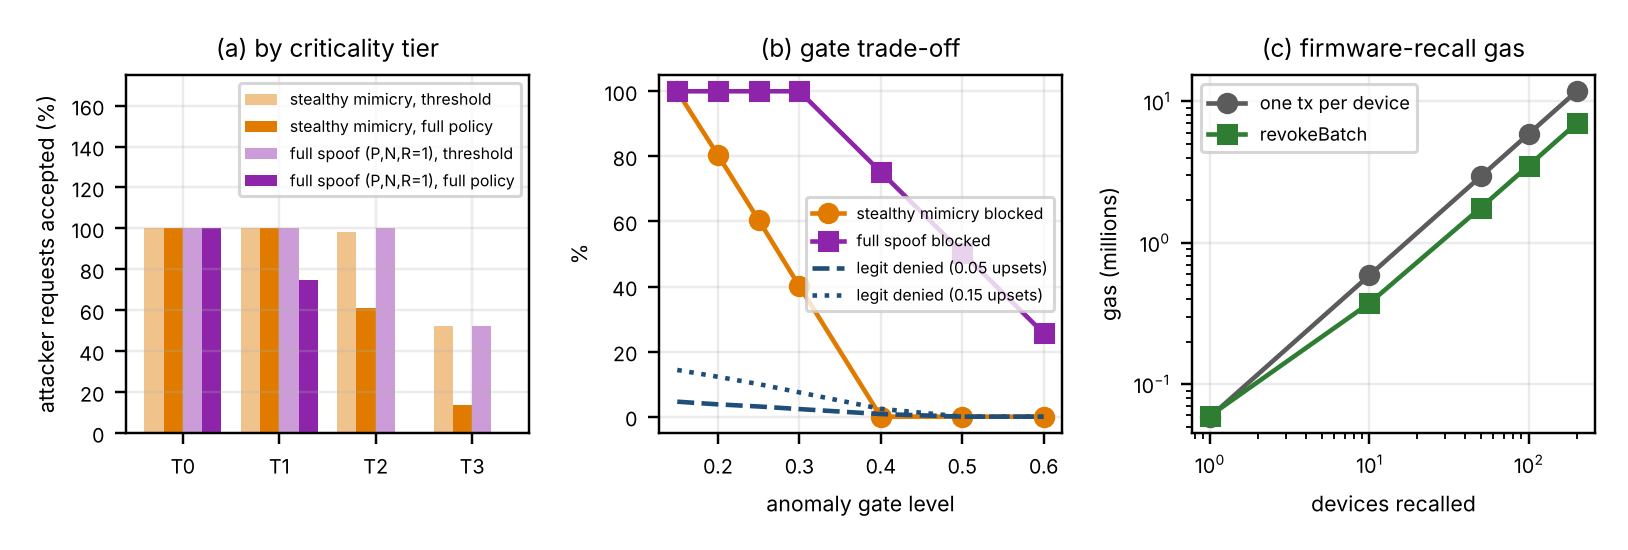
\includegraphics[width=0.86\textwidth]{../figures/fig8_iiot_results.png}
\caption{Industrial extensions: (a) attacker requests accepted per criticality tier under threshold-only and full policy; (b) anomaly-gate trade-off for 5\% and 15\% legitimate process-upset rates; (c) gas to recall devices with one transaction per device versus \texttt{revokeBatch}.}
\label{fig:iiotres}
\end{figure*}

\subsection{A Second Dataset: WUSTL-IIOT-2018 (SCADA)}\label{sec:wustl_eval}
To check that the gate behaviour is not specific to one collection, we repeat the policy experiment on WUSTL-IIOT-2018, flow records captured on a SCADA testbed with injected attacks \cite{teixeira2018scada,teixeira2018wustl}. The file has 7{,}037{,}983 rows and seven columns but only 62{,}959 distinct rows (99.1\% duplicates; 39{,}817 normal and 23{,}142 attack), and it carries a binary label only. Two consequences follow. First, de-duplication is essential: a random split of the raw file puts identical records in training and test data. Second, there are no attack types, so the held-out-type test of Section~\ref{sec:real_eval} cannot be repeated. We exclude the source port, as before, which leaves five count features (total, source and destination packets, total and source bytes), and use a stratified 70/30 split on the unique rows over five seeds.

A gradient-boosted classifier is almost perfect (AUC 0.99998, sd $2\times10^{-5}$): attack flows in this testbed are short (a median of two packets, at most 22) and normal flows are not, so the task is nearly trivial and the result says little about hard attacks. An Isolation Forest trained on normal flows only reaches AUC $0.909\pm0.006$, a more realistic stand-in for an attack never seen in training. For the policy we map the Isolation Forest score to $A\in[0,1]$ using normal training data alone (median to the 99.9th percentile), so no attack information enters the calibration.

Table~\ref{tab:wustl} gives the results. With the supervised score the full policy accepts at most 0.3\% of attack requests at T1--T3 and denies at most 0.2\% of legitimate ones, essentially the TON\_IoT picture. With the unsupervised score the gate and strict mode still reduce attack acceptance at the two critical tiers from 100\% and 94.1\% (threshold only) to 8.2\% and 4.3\%, but legitimate allowance drops to 87.5\% at T2 and 82.2\% at T3, a cost far above the 1--2\% seen with the supervised detector, because many normal flows look unusual to a detector fitted on five coarse counters. At T0 and T1 the unsupervised variant accepts all attack requests: the T1 gate is 0.60, above the median attack score of about 0.49. For an adaptive attacker that sends only its best 10\% (1\%) of flows, acceptance with the unsupervised score is 86.9\% (100\%) at T2 and 43.0\% (100\%) at T3, against 2.1\% (16.0\%) and 0.7\% (6.3\%) with the supervised score. A gate sweep with the unsupervised score shows the same trade-off as before: a gate of 0.3 denies 12.5\% of legitimate flows and blocks 91.3\% of attack flows, and a gate of 0.5 blocks none. The finding that carries over is the role of the gate; the finding that does not is that a strong detector is available. When the detector is weak, as an unsupervised one on coarse features is, the policy trades a large share of legitimate availability for protection at the critical tiers. As with TON\_IoT, posture and network context are synthetic and the flow-to-device pairing is arbitrary.

\begin{table}[t]
\centering
\caption{WUSTL-IIOT-2018: legitimate requests allowed and attack requests accepted (\%) under the threshold-only and full policies, for two sources of the anomaly signal}
\label{tab:wustl}
\scriptsize
\setlength{\tabcolsep}{2.5pt}
\begin{tabular}{@{}lrrrrrr@{}}
\toprule
 & \multicolumn{3}{c}{Supervised $A$} & \multicolumn{3}{c}{Isolation Forest $A$} \\
\cmidrule(lr){2-4}\cmidrule(lr){5-7}
Tier & Legit & Att.\ thr. & Att.\ full & Legit & Att.\ thr. & Att.\ full \\
\midrule
T0 & 100.0 & 100.0 & 100.0 & 99.3 & 100.0 & 100.0 \\
T1 & 100.0 & 100.0 & 0.1 & 97.1 & 100.0 & 100.0 \\
T2 & 100.0 & 0.3 & 0.3 & 87.5 & 100.0 & 8.2 \\
T3 & 99.8 & 0.2 & 0.1 & 82.2 & 94.1 & 4.3 \\
\bottomrule
\end{tabular}
\end{table}

\subsection{A Third Dataset With Attack Types: WUSTL-IIoT-2021}\label{sec:wustl21_eval}
WUSTL-IIoT-2021 contains Argus flow records from an industrial testbed running Modbus traffic, with four labelled attack types \cite{zolanvari2019vulnerability,zolanvari2021wustl}. It lets us repeat the held-out-type test that the SCADA file of Section~\ref{sec:wustl_eval} could not support. The file has 1{,}194{,}464 rows, 1{,}107{,}448 of them normal and the rest DoS (78{,}305), reconnaissance (8{,}240), command injection (259) and backdoor (212). All records were captured on one day, attacks come from two to four source hosts, and one column (\texttt{IdleTime}) is an epoch timestamp that separates attack types by capture time. We therefore drop timestamps, IP addresses, the source port, \texttt{IdleTime} and the IP-identification fields, keeping 39 features, and then remove 41{,}645 exact duplicates before splitting (1{,}152{,}819 rows remain). The evaluation follows Section~\ref{sec:real_eval}: a stratified 70/30 split over five seeds, a gradient-boosted classifier, an Isolation Forest trained on normal flows only (with $A$ calibrated on normal training scores alone, as before), and leave-one-type-out models as the held-out proxy.

\emph{Detection.} The supervised classifier is almost perfect on seen types (AUC 0.99999, and unchanged without the TTL fields, which fingerprint the attacker hosts). The Isolation Forest reaches AUC $0.987\pm0.001$, and between 0.983 and 0.990 for each attack type, because normal Modbus polling is very regular and the attacks (floods, scans) are far from it. Held-out detection is a different story: when DoS is removed from training, the classifier flags only 0.7\% of DoS test flows at 0.5 (AUC against normal 0.71), and for command injection and reconnaissance the figure is 8.1\% and 13.0\% although their AUC is above 0.999, which means the ranking is right but the scores sit far below any useful gate. Backdoor is found at 66.7\%. The command-injection and backdoor test sets contain only 74 and 63 flows, so those two figures are imprecise.

\emph{Policy.} Table~\ref{tab:wustl21} gives the full-policy results as means over the four attack types. With seen types the full policy admits 3.6--4.2\% of attack requests at T1--T3 (the average hides 10.8--12.1\% for backdoor and 3.8--4.5\% for command injection, the two rarest types) and denies none of the legitimate requests. With types withheld from training, acceptance rises to 75.4--77.8\% on average and to 97.9--99.2\% for DoS at the three higher tiers; the threshold-only policy is not much worse (last column), so on unseen types the supervised score contributes almost nothing, and an adaptive attacker sending its best 10\% or 1\% of flows is accepted in all cases. The unsupervised score behaves very differently on this data: the full policy admitted no attack request of any type at T1--T3, including the best 1\% of an adaptive attacker's flows, at the price of denying 1.5\%, 12.1\% and 22.3\% of legitimate requests at T1, T2 and T3. A gate of 0.5 on this score already blocks all attack flows while denying 2.3\% of legitimate ones, whereas the T2 and T3 gates (0.30 and 0.20) deny 12.0\% and 21.5\%. The two datasets with attack types therefore agree on the main point and disagree on the detector: a supervised detector does not protect against attack types it has not seen, and a detector trained on normal traffic only can, but only when normal traffic is as regular as it is in this testbed.

\emph{Limits of this result.} The favourable unsupervised numbers come from a laboratory testbed with machine-generated, nearly constant normal traffic and volumetric attacks from a handful of hosts, which makes anomaly detection easier than in a plant with operators, engineering workstations and maintenance windows. The rare attack types have very few flows, posture and network context are synthetic, and the pairing of a flow with a device is arbitrary.

\begin{table}[t]
\centering
\caption{WUSTL-IIoT-2021: legitimate requests allowed and attack requests accepted (\%) under the full policy, as means over four attack types; ``Thr.-only'' is the threshold-only policy on the held-out supervised scores}
\label{tab:wustl21}
\scriptsize
\setlength{\tabcolsep}{2.5pt}
\begin{tabular}{@{}lrrrrrr@{}}
\toprule
 & \multicolumn{3}{c}{Supervised $A$} & \multicolumn{2}{c}{Isolation Forest $A$} & \\
\cmidrule(lr){2-4}\cmidrule(lr){5-6}
Tier & Legit & Seen & Held-out & Legit & Attack & Thr.-only$^{a}$ \\
\midrule
T0 & 100.0 & 100.0 & 100.0 & 99.4 & 100.0 & 100.0 \\
T1 & 100.0 & 3.6 & 77.8 & 98.5 & 0.0 & 100.0 \\
T2 & 100.0 & 3.8 & 75.6 & 87.9 & 0.0 & 78.0 \\
T3 & 100.0 & 4.2 & 75.4 & 77.7 & 0.0 & 77.8 \\
\bottomrule
\end{tabular}
\end{table}

\subsection{Baseline Comparison: Revocation Exposure}\label{sec:baselines}
On a shared logical clock we compare the per-request design with a session token (HMAC bearer token, TTL 60 or 300\,s) and PKI with a CRL refreshed every 60 or 300\,s, for 60 devices at 1 request/s with revocation times drawn from $U(100,500)$\,s. Table~\ref{tab:base} shows that the audited design accepts no request after revocation, as Proposition~\ref{prop:revoke} predicts, whereas the baselines accept on average 33 and 147 requests for the 60\,s and 300\,s windows (worst cases 59--299). The mechanism implies this result; the experiment quantifies it. Token validation is the cheapest per request (an HMAC, no public-key operation) and our design costs more per accepted request, which we do not hide. The fast path trades the zero for a bounded exposure of at most $\rho\Delta$ requests (Proposition~\ref{prop:stale}): for example, with $\Delta=5$\,s and one request per second the bound is 5 requests, still far below the 33--147 of token and CRL schemes.

\begin{table}[t]
\centering
\caption{Revocation exposure (requests accepted after revocation; 60 devices, 1 req/s) and mean decision latency}
\label{tab:base}
\scriptsize
\begin{tabular}{@{}lrrr@{}}
\toprule
\textbf{Scheme} & \textbf{Mean exp.} & \textbf{Max exp.} & \textbf{Lat. (ms)} \\
\midrule
Session token (TTL 60 s) & 32.5 & 59 & 0.005 \\
Session token (TTL 300 s) & 146.5 & 299 & 0.006 \\
PKI$+$CRL (refresh 60 s) & 33.5 & 60 & 0.074 \\
PKI$+$CRL (refresh 300 s) & 146.5 & 299 & 0.094 \\
\textbf{Proposed (per-request)} & 0.0 & 0 & 0.070 \\
\bottomrule
\end{tabular}
\end{table}

Three further baselines address the objection that tokens and CRLs are weak comparators (Table~\ref{tab:base2}; 30 runs on the same revocation times, 60 devices, 1 request/s). Short-lived certificates with lifetime $L$ and OCSP stapling with response validity $V$ both bound exposure by the validity window, because a revoked device simply cannot renew; in our logical-clock model the two have identical exposure (29.0 requests for a 60\,s window, 140.8 for 300\,s) and differ only in who must be online (the CA for renewal, the responder for refresh), so we report them as the same mechanism and do not claim that one is better. A centralised online policy decision point that checks a revocation database on every request matches the proposed audited path with zero exposure, so exposure alone does not favour the blockchain design against this baseline. The differences are elsewhere: the central PDP is a single operator who alone can revoke, reinstate or silently alter its log; if it is unreachable for 60\,s it must either deny every request (86.7\% of legitimate requests served) or accept requests from devices revoked in the meantime (21.0 on average, up to 60); and its decision log has no external anchor. Our fast path faces the same outage trade-off for revocations that happen while the replica is blind (Section~\ref{sec:outage_eval}), so the claim we can support is about governance and auditability, not availability. The simulation models validity windows only; real deployments add renewal failures, clock skew and responder caching that we did not model.

\begin{table}[t]
\centering
\caption{Additional baselines: requests accepted after revocation and availability of legitimate requests (30 runs, 60 devices, 1 req/s)}
\label{tab:base2}
\scriptsize
\setlength{\tabcolsep}{2.5pt}
\begin{tabular}{@{}lrrr@{}}
\toprule
\textbf{Scheme} & \textbf{Mean exp.} & \textbf{Max exp.} & \textbf{Avail. (\%)} \\
\midrule
Short-lived cert (lifetime 60 s) & 29.0 & 60 & 100.0 \\
Short-lived cert (lifetime 300 s) & 140.8 & 300 & 100.0 \\
OCSP stapling (validity 60 s) & 29.0 & 60 & 100.0 \\
OCSP stapling (validity 300 s) & 140.8 & 300 & 100.0 \\
Central PDP (online, no outage) & 0.0 & 0 & 100.0 \\
Central PDP, 60 s outage, fail-closed & 0.0 & 0 & 86.7 \\
Central PDP, 60 s outage, fail-open & 21.0 & 60 & 100.0 \\
\bottomrule
\end{tabular}
\end{table}

\subsection{Firmware Recall Capacity}\label{sec:recall_eval}
Table~\ref{tab:recall} reports gas for revoking $k$ devices with one transaction each and with \texttt{revokeBatch} on the EVM; \texttt{suspendBatch} is shown for quarantine. For a single device the batch call is 1.7\% more expensive because of the loop and array overhead, but from ten devices on it saves 36.5--40.5\%, approaching about 35k gas per device against 58.9k. Taking a 30M-gas block, recalling $10^4$ devices needs about 20 blocks with individual transactions and 12 with batches, and $5\times10^4$ devices need 99 and 59 blocks (derived from the measured per-device gas; other traffic and block interval are not modelled, so at a 2\,s block time the larger recall would take on the order of two minutes at best). Revoking the highest-criticality devices first is therefore worth doing: devices revoked in later blocks stay exposed until their block.

\begin{table}[t]
\centering
\caption{Gas for recalling devices: one transaction per device versus \texttt{revokeBatch}, and \texttt{suspendBatch}}
\label{tab:recall}
\scriptsize
\begin{tabular}{@{}rrrrr@{}}
\toprule
Devices & One tx each & \texttt{revokeBatch} & Saving & \texttt{suspendBatch} \\
\midrule
1 & 58{,}862 & 59{,}885 & -1.7\% & 31{,}626 \\
10 & 588{,}584 & 373{,}727 & 36.5\% & 98{,}895 \\
50 & 2{,}943{,}016 & 1{,}768{,}639 & 39.9\% & 397{,}963 \\
100 & 5{,}886{,}008 & 3{,}512{,}255 & 40.3\% & 771{,}729 \\
200 & 11{,}772{,}196 & 6{,}999{,}571 & 40.5\% & 1{,}519{,}225 \\
\bottomrule
\end{tabular}
\end{table}

\subsection{Attack Detection}\label{sec:attacks}
Four basic attacks were run in 500 independent trials each: replay, forged signature, use after revocation and probing with unregistered DIDs. All were denied in every trial. With 500 trials and no failure the one-sided 95\% upper bound on the failure probability is $3/500=0.6\%$ (rule of three). This validates the state-machine logic against the implemented attacks; it is not evidence of unconditional security.

\subsection{Decentralized Revocation Governance}\label{sec:governance_eval}
Table~\ref{tab:governance} evaluates \texttt{RevocationGovernance} for $N\in\{5,7,9,11,15,21\}$ with 200 trials per size. Mean quorum latency on the testbed grows roughly linearly, from 0.56\,ms ($N=5$) to 1.91\,ms ($N=21$) for a cooperative group and from 0.93 to 3.67\,ms under maximal tolerated dissent ($N-q$ DENY voters), with 95\% CI half-widths of at most 0.10\,ms. Across all 1{,}200 trials the dissenting minority never prevented approval, and in 1{,}200 forced-revocation attempts with only $q-1$ approvals no revocation executed, consistent with Proposition~\ref{prop:gov}. On the EVM a proposal costs 72k gas, each vote 78k, and the final vote that triggers revocation 102k, so a quorum revocation costs 313k ($N=5$) to 800k gas ($N=21$): the governance cost grows with $q$, not with the fleet. Kumar et al.\ report 3--4\,s for registration and under 5\,s for revocation on a live PoA chain \cite{kumar2026privacy}; our figures are two to three orders of magnitude lower but measure compute only and are not comparable like for like. In a deployment each vote is a transaction, so revocation takes about $q$ block confirmations when votes are sequential, or one to two blocks if voters submit in parallel.

\begin{table}[t]
\centering
\caption{Governance: mean testbed latency (ms) cooperative and under maximal dissent; \% trials where maximal dissent still reached quorum (Appr.); \% where a $q-1$ coalition executed a revocation (Forced); EVM gas for one quorum revocation}
\label{tab:governance}
\scriptsize
\begin{tabular}{@{}rrrrrrr@{}}
\toprule
$N$ & $q$ & Coop. & Dissent & Appr.\% & Forced\% & Total gas \\
\midrule
5 & 3 & 0.562 & 0.926 & 100 & 0 & 313{,}402 \\
7 & 4 & 0.667 & 1.166 & 100 & 0 & 374{,}232 \\
9 & 5 & 0.803 & 1.440 & 100 & 0 & 435{,}062 \\
11 & 6 & 0.946 & 1.729 & 100 & 0 & 495{,}892 \\
15 & 8 & 1.299 & 2.438 & 100 & 0 & 617{,}552 \\
21 & 11 & 1.909 & 3.665 & 100 & 0 & 800{,}042 \\
\bottomrule
\end{tabular}
\end{table}

\subsection{End-to-End Evaluation on a Four-Validator QBFT Network}\label{sec:besu_eval}
To move beyond in-process execution we deployed the three contracts on a private Hyperledger Besu 25.7.0 network of four validators running QBFT with a 2\,s block period, a 4\,s round-change timeout, chain ID 2026 and zero base fee, and drove it through JSON-RPC with signed transactions (\texttt{besu\_benchmark.js}, \texttt{besu\_fault.js}). In this first deployment all four validators and the load generator ran on the same two-vCPU container, so the network is real in the sense that blocks are proposed, voted on and committed by separate processes, but there is no wide-area delay and the processes compete for the same two cores. The numbers below therefore describe consensus-bound behaviour on a small host; Section~\ref{sec:gcp_eval} repeats them across regions.

\textit{Latency and finality.} Table~\ref{tab:besu} shows that every state-changing call needs about one block period from submission to receipt (1.98--2.00\,s on average, p95 about 2.2\,s), independent of the operation; QBFT finalizes in the block that includes the transaction, so a receipt is also a final result. Revocation became visible when queried on a second validator after 1.87\,s on average, and 30 of 30 audited \texttt{evaluateAccess} calls issued after that point returned DENY. The measured difference between the submitting node's receipt and the replica's view was $-117\pm75$\,ms (the replica was seen to be up to date before the receipt poll returned, the maximum being +27\,ms), which is within our polling jitter of a few milliseconds to tens of milliseconds. We therefore read the replica lag as $\Delta\approx 0$ relative to the block period on a single host and, for the exposure bound $\rho\Delta$ of Proposition~\ref{prop:stale}, take the block period as the dominant term for the time between a revocation request and its enforcement.

\textit{Throughput.} Table~\ref{tab:besu2} reports audited decisions sent as pre-signed transactions from ten sender accounts. All transactions were mined at the three offered loads, but sustained throughput was 11--18 tx/s and latency grew with the queue (mean 31.6\,s at 600 offered). This is 12--19 times below the gas-based ceiling of about 213 decisions per second implied by 426 decisions per 30M-gas block at 2\,s, and the ceiling quoted in Section~\ref{sec:gas} should be read as an upper bound, not an estimate. We attribute the gap to CPU saturation (four JVMs and the load generator on two cores, with signature recovery and EVM execution for every transaction), but we did not profile it; the multi-region run of Section~\ref{sec:gcp_eval} gave higher throughput, which is consistent with this explanation without proving it. The practical consequence for the design is unchanged and strengthened: routine requests must not be sent through consensus.

\begin{table}[t]
\centering
\caption{Four-validator QBFT network (Besu 25.7.0, 2\,s blocks, single host): latency, finality and quorum revocation}
\label{tab:besu}
\scriptsize
\setlength{\tabcolsep}{2.5pt}
\begin{tabular}{@{}lrrr@{}}
\toprule
Measurement & Mean $\pm$ sd & p95 & $n$ \\
\midrule
Block interval (s) & 2.00 $\pm$ 0 & 2.00 & 40 \\
\texttt{register} submit$\to$receipt (ms) & 1977 $\pm$ 139 & 2165 & 40 \\
\texttt{evaluateAccess} submit$\to$receipt (ms) & 1997 $\pm$ 125 & 2179 & 40 \\
\texttt{anchorDecisions} submit$\to$receipt (ms) & 1993 $\pm$ 127 & 2185 & 20 \\
Revocation submit$\to$receipt (ms) & 1985 $\pm$ 121 & 2153 & 30 \\
Revocation submit$\to$visible on 2nd validator (ms) & 1868 $\pm$ 85 & 2018 & 30 \\
Quorum revocation, $N{=}5,q{=}3$, sequential votes (ms) & 8067 $\pm$ 237 & 8680 & 10 \\
Quorum revocation, $N{=}5,q{=}3$, parallel votes (ms) & 4033 $\pm$ 116 & 4156 & 10 \\
\bottomrule
\end{tabular}

\end{table}

\begin{table}[t]
\centering
\caption{Throughput of audited decisions on the same network (10 senders, pre-signed)}
\label{tab:besu2}
\scriptsize
\setlength{\tabcolsep}{3pt}
\begin{tabular}{@{}rrrr@{}}
\toprule
Offered & Mined & Throughput & Mean latency \\
decisions & & (tx/s) & (s) \\
\midrule
100 & 100 & 17.8 & 5.4 \\
300 & 300 & 16.0 & 14.7 \\
600 & 600 & 11.3 & 31.6 (p95 50.8) \\
\bottomrule
\end{tabular}

\end{table}

\textit{Governance and recall.} With five voters and quorum three, a revocation completed in 8.07\,s when votes were submitted one after another (each waiting for its block, so about four blocks) and in 4.03\,s when the votes were submitted together (about two blocks); all 20 proposals ended in revocation. A batch of 50 devices was revoked in one transaction (1.77M gas) and confirmed after 2.95\,s, and a batch of 200 devices (7.00M gas) after 6.13\,s; sampled revocations were visible on another validator. By comparison, registering 200 devices one transaction at a time took 399\,s. The batch and parallel-vote results confirm that on a block-timed chain, the number of blocks rather than the number of transactions determines recall and governance latency.

\textit{Fault tolerance.} With four validators QBFT tolerates one fault. With one validator stopped, registration latency had a mean of 2.83\,s (sd 2.00\,s, p95 6.16\,s, $n=8$) against 1.97\,s at baseline: the median was unchanged (1.91\,s), but rounds in which the stopped validator was the proposer had to time out and change round. With two validators stopped no block was produced and a pending transaction was not mined within 20\,s; after both were restarted it was mined after 78\,s. These runs used a single pending transaction and small samples, so they show the qualitative behaviour (safe halt below the quorum, resumption after recovery) rather than a tight latency estimate. For the architecture, they mean that the fast path keeps deciding on its last replicated state during a halt and the outage policy of Section~\ref{sec:outage} governs what is allowed meanwhile.

\subsection{Four Validators in Four Regions}\label{sec:gcp_eval}
To remove the shared-CPU limitation and add real network distance, we repeated the same benchmark on Google Cloud with one validator per e2-standard-2 virtual machine (2 vCPU, 8\,GB) in europe-west3, us-east4, asia-southeast1 and southamerica-east1 (same Besu 25.7.0 and QBFT parameters as above; Ubuntu 24.04 and OpenJDK 21). The load generator ran in europe-west3 and submitted through the European validator's endpoint; the revocation-visibility test queried two validators in other regions (endpoints 3 and 4 in the run configuration, which are the Asian and South American ones). We injected no artificial delay and did not record round-trip times, so the delay is whatever the provider's inter-region network gave on the day of the run (2026-10-12). Table~\ref{tab:gcp} sets the results next to the single-host run. Both are single runs of the same script, with the sample sizes of Table~\ref{tab:besu}.

\textit{Finality and latency.} Block production stayed at 2.00\,s with no deviation, and the latency of \texttt{register}, \texttt{evaluateAccess} and \texttt{anchorDecisions} was unchanged within noise (1.98--2.00\,s, p95 2.16--2.18\,s). Consistent with this, inter-region distance did not push consensus beyond one block period on this network; the 2\,s timer, not the network, set finality. The revocation receipt took 1.55\,s on average, less than on one host; we did not investigate this, the submissions are not aligned to the block timer, and we do not read it as a speed-up.

\textit{Replica lag.} A revocation became visible on a validator in another region 1.76\,s after submission, and 30 of 30 audited decisions on a second remote validator issued afterwards returned DENY. Unlike on one host, the replica now trailed the receipt: by $+212\pm145$\,ms on average (p95 362\,ms, maximum 495\,ms, minimum $-39$\,ms). Taking the largest value as an estimate for this network, the time between a revocation request and its visibility to a remote replica was about one block period plus 0.2--0.5\,s, so the exposure bound $\rho\Delta$ of Proposition~\ref{prop:stale} for a fast-path gateway is dominated by the block period but no longer negligible against the network. This is one run on one provider's backbone; a plant link over a public network or a satellite path would give a larger $\Delta$ and has to be measured where it is deployed.

\textit{Throughput.} All 100, 300 and 600 pre-signed audited decisions were mined, at 30.8, 34.4 and 50.1 tx/s, against 17.8, 16.0 and 11.3 on one host; the mean latency at 600 offered fell from 31.6\,s to 8.6\,s (p95 10.7\,s). This is consistent with the CPU contention suspected earlier, but throughput still rose with offered load, so we did not find the saturation point, and a figure of 50 tx/s is a lower bound for this deployment, not its capacity. It remains 4--7 times below the gas-based ceiling of 213 decisions per second. We did not determine what limits it (block gas, round timing or the load generator), and the conclusion for the design is unchanged: routine requests must not wait for consensus.

\begin{table}[t]
\centering
\caption{The same benchmark on one host and with one validator in each of four Google Cloud regions (mean $\pm$ sd; single runs)}
\label{tab:gcp}
\scriptsize
\setlength{\tabcolsep}{3pt}
\begin{tabular}{@{}lrr@{}}
\toprule
Measurement & One host & Four regions \\
\midrule
Block interval (s) & 2 $\pm$ 0 & 2 $\pm$ 0 \\
\texttt{register}, submit$\to$receipt (ms) & 1977 $\pm$ 139 & 1980 $\pm$ 162 \\
\texttt{evaluateAccess}, submit$\to$receipt (ms) & 1997 $\pm$ 125 & 1997 $\pm$ 134 \\
\texttt{anchorDecisions}, submit$\to$receipt (ms) & 1993 $\pm$ 127 & 1993 $\pm$ 130 \\
Revocation, submit$\to$receipt (ms) & 1985 $\pm$ 121 & 1552 $\pm$ 169 \\
Revocation, submit$\to$visible on replica (ms) & 1868 $\pm$ 85 & 1764 $\pm$ 211 \\
Replica minus receipt (ms) & -117 $\pm$ 75 & 212 $\pm$ 145 \\
Quorum revocation $N{=}5,q{=}3$, sequential (s) & 8.07 $\pm$ 0.24 & 8.17 $\pm$ 0.14 \\
Quorum revocation $N{=}5,q{=}3$, parallel (s) & 4.03 $\pm$ 0.12 & 4.33 $\pm$ 0.13 \\
\texttt{revokeBatch}, 50 devices, receipt (s) & 2.95 & 2.41 \\
\texttt{revokeBatch}, 200 devices, receipt (s) & 6.13 & 2.99 \\
Throughput, 100 offered (tx/s) & 17.8 & 30.8 \\
Throughput, 300 offered (tx/s) & 16.0 & 34.4 \\
Throughput, 600 offered (tx/s) & 11.3 & 50.1 \\
Mean latency at 600 offered (s) & 31.6 & 8.6 \\
\bottomrule
\end{tabular}
\end{table}

\textit{Governance and recall.} A three-of-five revocation took 8.17\,s with sequential votes and 4.33\,s with parallel votes (all 10 trials each ended in revocation), the same four and two blocks as on one host (8.07 and 4.03\,s). Revoking 50 and 200 devices in one transaction was confirmed after 2.41 and 2.99\,s for 1.77M and 7.00M gas, the same gas as before, and the sampled revocations were visible on another validator; the single-host run needed 2.95 and 6.13\,s. Registering the devices one by one still took 99.7\,s for 50 and 399\,s for 200, about one block each, so the argument for batching in Section~\ref{sec:recall} is unchanged.

\textit{Fault tolerance.} With one validator stopped, registration took $3.43\pm2.17$\,s (p50 2.14\,s, p95 6.29\,s, $n=8$) against 2.83\,s on one host; the median stayed near the baseline and the mean reflects the rounds in which the stopped validator was the proposer. With two validators stopped no block was produced and a pending transaction was not mined within 20\,s; after the validators were restarted it was mined after 75.0\,s (78\,s on one host). As before, these runs used one pending transaction and few samples and show the qualitative behaviour. We did not test network partitions, injected delay or validators in the same region.

\subsection{Static Analysis and Randomised Invariant Tests}\label{sec:assure}
We ran Slither on the three contracts with its 102 detectors. It reported 11 findings: one medium (a strict equality on \texttt{registeredAt==0} in \texttt{getStatus}, which is the intended existence test), four low (timestamp-comparison warnings on the same existence test and on a status check, a missing zero-address check on the oracle in the constructor, and an event emitted after the external registry call in \texttt{castVote}, whose callee is our own trusted registry), one informational finding per signature-recovery routine (inline assembly) and four optimisation hints (state variables that could be immutable). No reentrancy, access-control or arithmetic finding was reported. Reading the code for what Slither does not check, we found one genuine gap: if the oracle address were zero, or a device were registered with a zero signer, an invalid signature (for which \texttt{ecrecover} returns the zero address) would pass. We added a zero-oracle check in the constructor and rejected a zero recovered address at registration; the measured cost is +62 gas for \texttt{registerDevice} and none for the other operations. We did not apply the immutable hints, to keep the measured gas comparable across the evaluation. Signature malleability is harmless here because replay protection is keyed on (device, nonce), not on the signature bytes.

Three new tests complement the 13 unit tests: the zero-oracle and zero-signer cases, and a randomised state-machine test that applies 300 steps (three seeds, six devices) of suspend, reinstate, revoke and access operations against an independent model. It checks that revocation is terminal, that reinstatement succeeds only from the suspended state, that an inactive device or a reused (device, nonce) pair is never allowed, and that the on-chain status always equals the model status. All 16 tests pass. This is bounded random testing, not a proof and not an audit; the contracts have not been formally verified.

\subsection{Degraded Operation During an Outage}\label{sec:outage_eval}
Table~\ref{tab:outage} applies the policy of Section~\ref{sec:outage} to a scenario with 400 devices, one request per second each, a quarter of the devices acting as T2 clients that issue a T2 request every fourth second, and 10\% of the devices revoked at random times during an outage that starts at $t=200$\,s of 600\,s. A fully fail-closed PEP stops serving everyone for the whole outage, so availability falls to 89.9\% for a 60\,s outage and 50.4\% for 300\,s. The degraded policy keeps T0--T1 running (99.4\% and 97.0\%) but denies every T2 request during the outage and accepts requests from devices revoked while it was blind (962 requests for 60\,s, 4{,}398 for 300\,s). This scenario follows directly from the stated policy and is deterministic given its parameters, so it is an illustration of the trade-off, not an empirical result; its use is to show that the operator chooses between unsafe acceptances and lost availability, and that the choice is explicit.

\begin{table}[t]
\centering
\caption{Outage scenario (policy-defined, 400 devices, 1 req/s): availability of legitimate requests and unsafe accepts}
\label{tab:outage}
\scriptsize
\setlength{\tabcolsep}{2.5pt}
\begin{tabular}{@{}rrrrrr@{}}
\toprule
Outage & Revoked & \multicolumn{2}{c}{Avail.\ (\%)} & Unsafe & T2--T3 \\
(s) & devices & closed & degr. & accepts & denied \\
\midrule
10 & 43 & 98.3 & 99.9 & 155 & 100\% \\
30 & 40 & 94.9 & 99.7 & 456 & 100\% \\
60 & 36 & 89.9 & 99.4 & 962 & 100\% \\
120 & 44 & 79.7 & 99.0 & 2{,}149 & 100\% \\
300 & 30 & 50.4 & 97.0 & 4{,}398 & 100\% \\
\bottomrule
\end{tabular}
\end{table}
